\documentclass{beamer}

\usepackage[english]{babel}
\usepackage[utf8]{inputenc}
\usepackage[T1]{fontenc}
\usepackage{tikz}

\usetheme{nescala}
\setbeamercovered{transparent}

\newcommand\demoslide{
  {
    \setbeamertemplate{background}{}
    \begin{frame}[plain]
      \begin{center}\Large\bfseries Demo\end{center}
    \end{frame}
  }
}

\newcommand\fullpicture[1]{
  {
    \setbeamertemplate{background}{}
    \begin{frame}[plain]
      \begin{tikzpicture}[remember picture,overlay]
        \node[at=(current page.center)] {
          \includegraphics[keepaspectratio,height=1.2\paperheight,width=1.2\paperwidth]{#1}
        };
      \end{tikzpicture}
    \end{frame}
  }
}

\begin{document}

  \title{Macros vs Types}
  \author{Eugene Burmako \& Lars Hupel}
  \institute{\'Ecole Polytechnique F\'ed\'erale de Lausanne\\Technische Universit\"at M\"unchen}
  \date{March 1, 2014}

{
\setbeamertemplate{footline}{}
\begin{frame}
  \titlepage
\end{frame}
}

\begin{frame}{Macros vs types}
  \begin{itemize}
  \item Types have been used to metaprogram Scala for ages
  \item Macros are the new player on the field
  \item Debates are hot in the IRC and on Twitter
  \item Time to figure out who's the best once and for all!
  \end{itemize}
\end{frame}

\begin{frame}{Let the games begin!}
  Following the \text{\color{blue}\href{http://scalamacros.org/paperstalks/2014-02-04-WhatAreMacrosGoodFor.pdf}{"What are macros good for?"}} talk, we will see how the contenders fare in three disciplines:

  \vspace{1em}
  \begin{itemize}
  \item Code generation
  \item Static checks
  \item Domain-specific languages
  \end{itemize}
\end{frame}

\begin{frame}
\vskip40pt
\begin{center}
\text{\color{blue}{\Large{Code generation}}}
\end{center}
\end{frame}

\begin{frame}[fragile]
\frametitle{Code generation}
  Every language ecosystem has it\only<2>{, even Haskell
  \vspace{1em}
    \begin{itemize}
    \item \texttt{lens}

       derive lenses for fields of a data type
    \item \texttt{yesod}

      templating, routing
    \item \texttt{invertible-syntax}

      constructing partial isomorphisms for constructors
  \end{itemize}
  }
\end{frame}

\begin{frame}[fragile]{Textual code generation}{Example: Parser generators}
  % from Tom Niemann <epaperpress.com>
  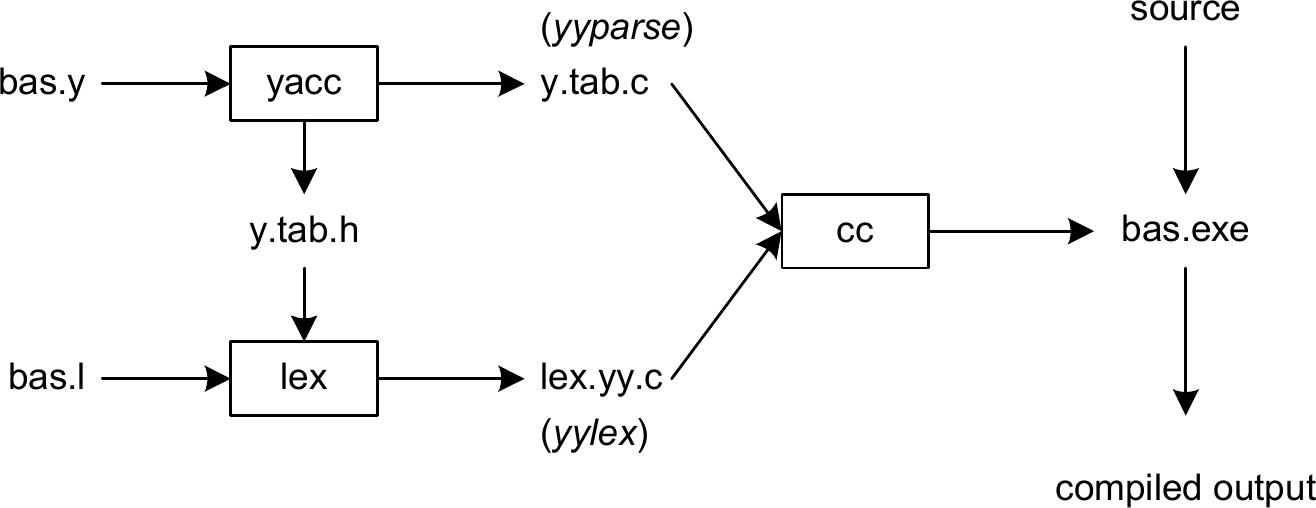
\includegraphics[width=\linewidth]{img/yacc.png}
\end{frame}

\begin{frame}[fragile]
\frametitle{Textual codegen is too low-tech}
  \begin{itemize}
  \item Easy to mess up when concatenating strings
  \item Little knowledge about the program being compiled
  \item We need a better solution!
  \end{itemize}
\end{frame}

\begin{frame}{Enter types}
  \begin{itemize}
  \item Scala's type system is Turing-complete
  \item This enables some form of code generation
  \item But it's not particularly straightforward
  \end{itemize}
\end{frame}

% Do we want to provide an example here?

\begin{frame}{Enter macros}
  \begin{itemize}
  \item Functions that are run at compile time
  \item Operate on abstract syntax trees not on strings
  \item Communicate with compiler to learn things about the program
  \item A lot of popular Scala libraries are already using macros
  \end{itemize}
\end{frame}

\begin{frame}[fragile]{Use case: Specialization}
  Specialization helps with writing high-performance code,
  but it bloats the code significantly.

  \vspace{1em}
  \begin{verbatim}
def createArray[@specialized T](size: Int, el: T) = {
  val a = new Array[T](size)
  for (i <- 0 until size) a(i) = el
  a
}
  \end{verbatim}
\end{frame}

\begin{frame}[fragile]{Use case: Specialization}
  With macros we can write a specialization code generator ourselves,
  having fine-grained control over what we're specializing.

  \vspace{1em}
  \begin{semiverbatim}
def specialized[T: ClassTag](code: => T) = macro ...

def createArray[T: ClassTag](size: Int, el: T) = \{
  val a = new Array[T](size)
  \text{\color{blue}{specialized[T] \{}}
    for (i <- 0 until size) a(i) = el
  \text{\color{blue}{\}}}
  a
\}
  \end{semiverbatim}
\end{frame}

\begin{frame}{Macros + types}
  \begin{itemize}
  \item With macros code generation becomes acessible and fun
  \item But we don't have to do that mindlessly
  \item Types make things better
  \item And metaprogramming is not an exception
  \end{itemize}
\end{frame}

\begin{frame}{Use case: Materialization}
  We want to have: default implementations for
  \begin{itemize}
    \item \texttt{\color{red}{Semigroup}} (pointwise addition)
    \item \texttt{Ordering} (lexicographic order)
    \item \texttt{Binary} (pickling/unpickling)
  \end{itemize}

  \vspace{1em}
  We do not want to: write boilerplate
  \begin{itemize}
    \item repetitive \& error-prone
  \end{itemize}
\end{frame}

\begin{frame}{Use case: Materialization}
  \texttt{scalac} already synthesizes \texttt{equals}, \texttt{toString} ...

  \vspace{1em}
  \begin{alertblock}{Problem}
    Not extensible
  \end{alertblock}

  \vspace{1em}
  \begin{exampleblock}{Solution}
    Materialization based on type classes and implicit macros
  \end{exampleblock}
\end{frame}

\begin{frame}{Type classes \'a la Scala}
  \begin{itemize}
    \item Type classes are (first-class) traits
    \item Instances are (first-class) values
    \item<visible@2> Both can use arbitrary language features
  \end{itemize}
\end{frame}

\begin{frame}[fragile]{Use case: Materialization}
  \begin{verbatim}
implicit def derive[C[_] : TypeClass, T]: C[T] =
  macro TypeClass.derive_impl[C, T]
  \end{verbatim}
\end{frame}

% \demoslide

\begin{frame}{The power of materialization}
  \begin{itemize}
    \item First introduced in Shapeless
    \item Similar to \texttt{deriving Eq} in Haskell
    \item Extensible without modifying the macro(s) itself
  \end{itemize}
\end{frame}

\begin{frame}[fragile]{The dangers of materialization}
  \vspace{1em}
  \begin{alertblock}{Bad}
  \begin{verbatim}
implicit def derive[C[_], T]: C[T] =
  macro TypeClass.derive_impl[C, T]
  \end{verbatim}
  \end{alertblock}

  \vspace{1em}
  \begin{exampleblock}{Good}
  \begin{semiverbatim}
implicit def derive[C[_] : \text{\color{blue}{TypeClass}}, T]: C[T] =
  macro TypeClass.derive_impl[C, T]
  \end{semiverbatim}
  \end{exampleblock}
\end{frame}

\begin{frame}[fragile]
\frametitle{Our advice}
  \begin{itemize}
    \item Metaprogramming is powerful
    \item But it is also hard, so prefer programming
    \item Try to constrain the types of the macros as much as possible
    \item Try to encapsulate only the ``moving parts'' into a macro

      (maybe more boilerplate, but more predictable)
  \end{itemize}
\end{frame}

% \begin{block}{Open problems}
%   Best practices for documentation \& testing
%   \vspace{1em}
%   Do we need a compile-time ScalaCheck?
% \end{block}

\begin{frame}
\vskip40pt
\begin{center}
\text{\color{blue}{\Large{Static checks}}}
\end{center}
\end{frame}

\begin{frame}{Types \'a la Pierce}
  \begin{quote}
    ``A type system is a tractable syntactic method for \alert<2>{proving the absence of certain program behaviors} by classifying phrases according to the kinds of values they compute.''
  \end{quote}
  \hfill -- Benjamin Pierce, in: Types and Programming Languages
\end{frame}

\begin{frame}{Types \'a la Scala}
  Scala has a sophisticated type system
  \begin{itemize}
    \item Path-dependent types
    \item Type projections
    \item Higher-kinded types
    \item Implicit parameters
  \end{itemize}
\end{frame}

\begin{frame}{Type computations}
  Implicits allow computations in the type system

  \begin{itemize}
    \item Higher-order unification (SI-2712)
    \item Generic operations on tuples
    \item Extensible records
    \item Statically size-checked collections
  \end{itemize}
\end{frame}

\begin{frame}{Shapeless}
  The library that makes advanced types accessible!
\end{frame}

\begin{frame}[fragile]{Type computations}{Example: Sized collections}
  \begin{verbatim}
// typed as Sized[_2, List[String]]
val hdrs = Sized("Title", "Author")

// typed as List[Sized[_2, List[String]]]
val rows = List(
  Sized("TAPL", "B. Pierce"),
  Sized("Implementation of FP Languages", "SPJ")
)
  \end{verbatim}

  \color{red}{Maybe collection operation on tuples or records? These are my personal favorites in Shapeless.}
\end{frame}

% \demoslide

\begin{frame}{The power of type computation}
  Computing with implicits is sometimes called ``Poor Man's Prolog''
  \vspace{1em}

  But: Almost anything can be done

  \color{red}{Not sure whether I follow}
\end{frame}

% <https://secure.flickr.com/photos/mszeto/3261725397/>
\fullpicture{img/hanoi.jpg}

\begin{frame}{How can macros help?}
  \begin{itemize}
    \item Type system doesn't cover everything
    \item Complex type computations are hard to debug

      (sometimes, \texttt{-Xlog-implicits} is not enough)
    \item Implicit-heavy code slows down compiler significantly
  \end{itemize}
\end{frame}

\begin{frame}[fragile]{Let's overthrow the tyranny of types!}
  Macros can do anything, including validation of arguments,
  so we shouldn't bother with all those complex types anymore

  \vspace{1em}
  \begin{alertblock}{Bad}
  \begin{verbatim}
trait GenTraversableLike[+A, +Repr] {
  def map[B, That](f: A => B)
    (implicit bf: CanBuildFrom[Repr, B, That]): That
}\end{verbatim}
  \end{alertblock}

  \begin{exampleblock}{Good}
  \begin{semiverbatim}
trait GenTraversableLike \{
  def map(f: Any => Any): Any = \text{\color{blue}{macro}} impl
\}
  \end{semiverbatim}
  \end{exampleblock}
\end{frame}

\begin{frame}[fragile]{Let's overthrow the tyranny of types... NOT!}
  \begin{center}
    % from https://upload.wikimedia.org/wikipedia/commons/7/79/Operation_Upshot-Knothole_-_Badger_001.jpg
    
\includegraphics[height=8cm]{img/boom.jpg}
  \end{center}
\end{frame}

\begin{frame}[fragile]{Sane use case: Checked arithmetics}
  Spire provides a \texttt{checked} macro to detect arithmetic overflows.
  Types can't capture this, so it's okay to use a macro here.

  \vspace{1em}
  \begin{verbatim}
// returns None when x + y overflows
Checked.option {
  x + y < z
}
  \end{verbatim}
\end{frame}

\begin{frame}{Sane use case: Example of short-circuiting computations with macros}
  What would be the best example from shapeless here?
\end{frame}

\begin{frame}{Our advice}
  \begin{itemize}
  \item Types whenever possible
  \item Macros if impossible or heavyweight
  \item Type classes to encapsulate the magic
  \end{itemize}
\end{frame}

\begin{frame}
\vskip40pt
\begin{center}
\text{\color{blue}{\Large{Domain-specific languages}}}
\end{center}
\end{frame}

\begin{frame}
\vskip40pt
\begin{center}
\text{\color{blue}{\Large{Summary}}}
\end{center}
\end{frame}

\end{document}
